\section{Internet das coisas}
\label{sec:iot}
A Internet nesta última década tem contribuído de forma significativa na economia e sociedade, deixando como legado uma notável infraestrutura de rede de comunicação. O seu maior disseminador nesse período, vem sendo \textit{World Wide Web}(WWW), o qual permite o compartilhamento de informação e mídia de forma global\cite{Chandrakanth:2014}.

No âmbito da economia, por exemplo, o E-Commerce permitiu potencializar as vendas de produtos e serviços, com um faturamento estimado para o ano de 2016 de aproximadamente 56,8 bilhões de reais no Brasil, segundo ecommercenews\footnotemark \footnotetext{https://ecommercenews.com.br/noticias/pesquisas-noticias/e-commerce-brasileiro-deve-crescer-18-e-faturar-r-568-bilhoes-em-2016}. Além do benefício direto para sociedade provindo do E-Commerce, onde as pessoas podem realizar pesquisa de preços de serviços e produtos e, adquiri-los de forma comoda, sem precisar se deslocar até um ponto de venda, a Internet dispõe para a sociedade diversas outras oportunidades, como cursos a distância oferecidos por diversas universidades de todo o mundo, a exemplo dos cursos disponibilizados pela plataforma Coursera\footnotemark \footnotetext{\url{https://pt.coursera.org/}}. 

A Internet está se tornando cada vez mais persistente no cotidiano, devido, por exemplo, ao crescente número de usuários de dispositivos móveis, os quais possuem tecnologias de conexão com a Internet, as quais cada dia tornam-se mais acessíveis (presentes em locais que não tinham e, mais baratas)\cite{Chandrakanth:2014}.

Em 2010 havia aproximadamente 1,5 bilhão de PCs conectados a Internet e mais que 1 bilhão de telefones móveis\cite{Sundmaeker:2010}. Segundo Gartner\footnotemark \footnotetext{\url{http://www.gartner.com/newsroom/id/3165317}}, 6,4 bilhões de coisas estarão conectadas até o final de 2016 e, em 2020 esse número atingirá cerca de 20,8 bilhões. A previsão de \cite{Sundmaeker:2010}, a qual dizia que a denominada Internet dos PCs seria movida para o que se chama de Internet das Coisas fica então mais evidente neste atual cenário.

A ideia básica da \textit{Internet of things (IoT)}, traduzido para o português como Internet das Coisas é a presença pervasiva de uma variedade de "coisas ou objetos", tais como RFID tags, sensores, telefones móveis, dentre outros. Os quais, através de esquemas de endereçamento único são capazes de interagir com os outros e cooperar com seus vizinhos para alcançar um objetivo em comum\cite{Atzori:2010}. Outros exemplos de "coisas ou objetos" podem ser pessoas, geladeiras, televisores, veículos, roupas, medicações, livros, passaportes, contanto que possam ser identificadas unicamente e possam se comunicar com as outras coisas e/ou possam ser acessados remotamente por humanos.

Dentre as diversas definições de Iot pode-se citar duas, a primeira define de maneira mais geral, tanto a atual realidade, quanto a prospeção futura. Já a segunda especifica melhor como deve ser o cenário ideal da Internet das Coisas, pois já embuti explicitamente os conceitos de capacidades de autoconfiguração, interoperabilidade e interfaces inteligentes.
\begin{enumerate}
\item Segundo\cite{iot2020:2008}, \textit{Internet of Things} significa rede mundial de objetos unicamente endereçáveis e interconectados, seguindo os protocolos dos padrões de comunicação.
\item IoT é parte integrante da futura Internet e pode ser definida como uma infraestrutura de rede global dinâmica com capacidades de autoconfiguração baseada nos padrões e interoperabilidade dos protocolos de comunicação onde coisas físicas e virtuais têm identidade, atributos físicos, personalidade virtual, usam interfaces inteligentes e, são integradas dentro da rede de informações \cite{Sundmaeker:2010}.
\end{enumerate}

Diante deste cenário da IoT, pode-se citar exemplos de aplicações em diversos domínios, tais como, logística e transporte; cuidados com a saúde; ambiente inteligente (casa (seção \ref{sec:hns}), escritório); dentre outros\cite{Atzori:2010}.

Apesar da grande potencialidade da Internet das Coisas, ainda existem muitos desafios a serem vencidos, como por exemplo a disponibilidade de uma interface de comunicação (acesso aos serviços e informações dos dispositivos) e programação comum aos objetos. A falta desta padronização faz com que se torne oneroso o desenvolvimento de aplicações para o objeto, pois cada coisa possui suas próprias interfaces, logo para cada dispositivo um desenvolvimento a parte. Mais difícil ainda é prover uma única funcionalidade ou serviço com a composição dos diversos objetos. Para diminuir a dificuldade deste cenário, pode-se disponibilizar os dispositivos como serviços WEB (seção \ref{subsec:dispositivosweb}), desta forma pode-se utilizar os protocolos WEB como linguagem comum de integração dos dispositivos a Internet.\cite{Franca:2011}

\subsection{Serviços web}
Segundo\cite{Dustdar:2005}, um serviço web é um sistema identificado por uma URL\footnotemark \footnotetext{Acrônimo para Uniform Resource Locator e é uma referência (um endereço) para um recurso na Internet.\cite{oracle:url}}, no qual suas interfaces públicas são definidas e descritas usando XML\footnotemark \footnotetext{Extensible Markup Language (XML) é uma simples e flexível linguagem de marcação utilizada para codificar documentos através de regras produzidas por humanos, as quais podem ser manipulados (compreendidas) por máquinas \cite{w3c:xml}\cite{w3c:xmlschema}} e, suas definições podem ser descobertas por outros sistemas. Sistemas então podem interagir com os serviços web utilizando suas definições e descrições. Através destas utiliza-se mensagens XML que são trasmitidas seguindo os protocolos padrão (definidos por W3C\footnotemark \footnotetext{\url{https://www.w3.org/}}) da Internet para que haja tal interação.

Um dos modelos (Figura \ref{fig:wsmodelwsdl}) utilizados por esses sistemas consiste em 3 camadas:
\begin{itemize}
\item Provedor (Provider) - cria ou oferece o serviço web, este precisa descrever o serviço em um formato padrão, neste caso XML e, publica-o no Registro de serviço.
\item Registro de serviço (Registry) - além da descrição do serviço, contém informações adicionais à respeito do provedor, como endereço e contato da empresa desenvolvedora do serviço e, detalhes técnicos. 
\item Consumidor (Consumer) - obtem informação do registro e utiliza a descrição do serviço capturada para invocar o serviço web.
\end{itemize}

\begin{figure}[!htb] \centering 
  \centering
  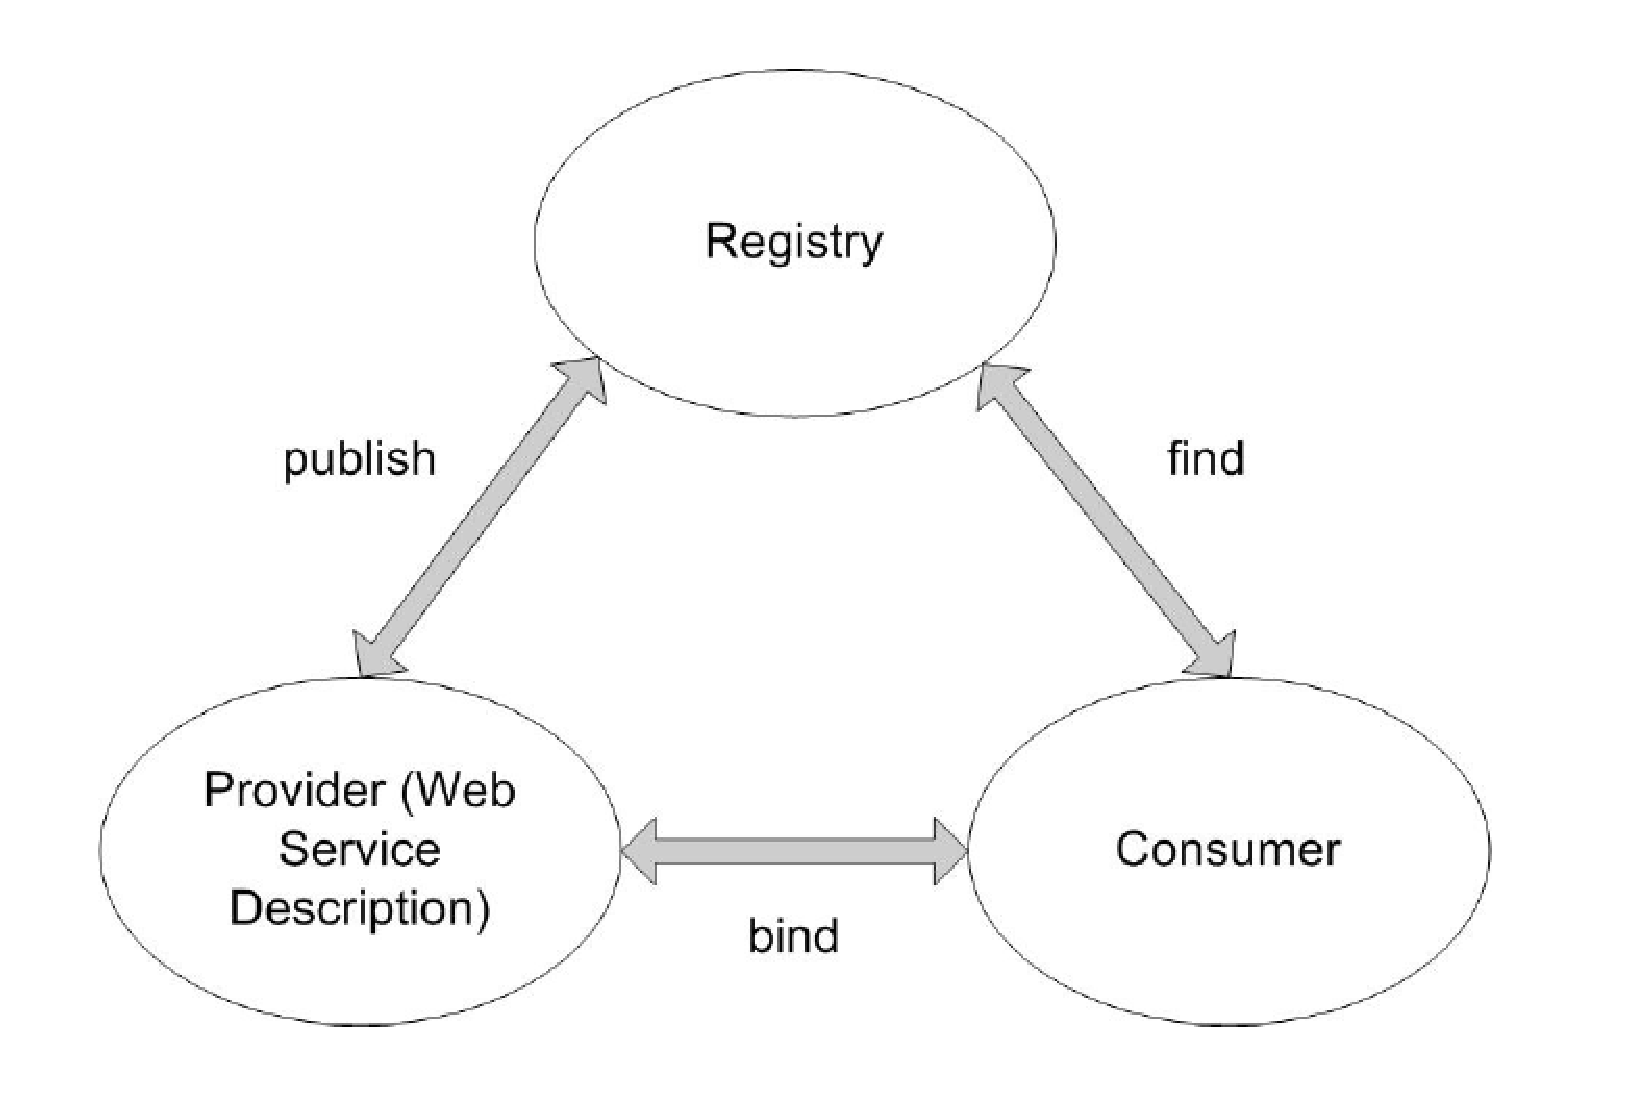
\includegraphics[width=0.8\columnwidth]{fundamentacao/webservice_model_wsdl} 
  \caption{Modelo de serviços web em 3 camadas.\cite{Dustdar:2005}} 
  \label{fig:wsmodelwsdl}
\end{figure}

Serviços web possuem baixo nível de acoplamento e utilizam padrões para oferecer suas funcionalidades, pois tais serviços tem a intenção de prover comunicação a diferentes tipos de aplicações, que possivelmente são executadas em diferentes plataformas. A \textit{Web Service Description Language}(WSDL) usa o formato XML para descrever os métodos oferecidos por um serviço web, incluindo parâmetros de entrada e saída, tipos de dados e, protocolo de transporte utilizado (normalmente o HTTP). O \textit{Simple Object Access Protocol}(SOAP, seção \ref{subsec:soap}) é utilizado para as trocas de mensagens (formatadas em XML) entre as entidades envolvidas no modelo de serviço web citado.\cite{Dustdar:2005}

\subsection{SOAP}
\label{subsec:soap}
...

\subsection{Princípios arquiteturais REST}
...
\subsection{Dispositivos como serviços web}
\label{subsec:dispositivosweb}
Como abordado em \ref{sec:iot} um dos desafios referente a visão da IoT é sua interoperabilidade e, como possível solução se pode utilizar dos existentes protocolos web. Desta maneira os dispositivos podem interagir entre si e com outros sistemas na web.

Adotando esse padrão, os dispositivos podem ter suas propriedades disponíveis através de qualquer navegador, sem a necessidade de instalação de nenhum programa ou driver adicional, como pode ser exemplificado na Figura \ref{fig:dispnavegador}. Além disto, mashups físicos** podem ser construídos com muito menos esforço do que as existentes abordagens, quebrando drasticamente a barreira para o desenvolvimento de aplicações com dispositivos, assim então promovendo a visão da Internet das Coisas.\cite{Guinard:2009}

\begin{figure}[!htb] \centering 
  \centering
  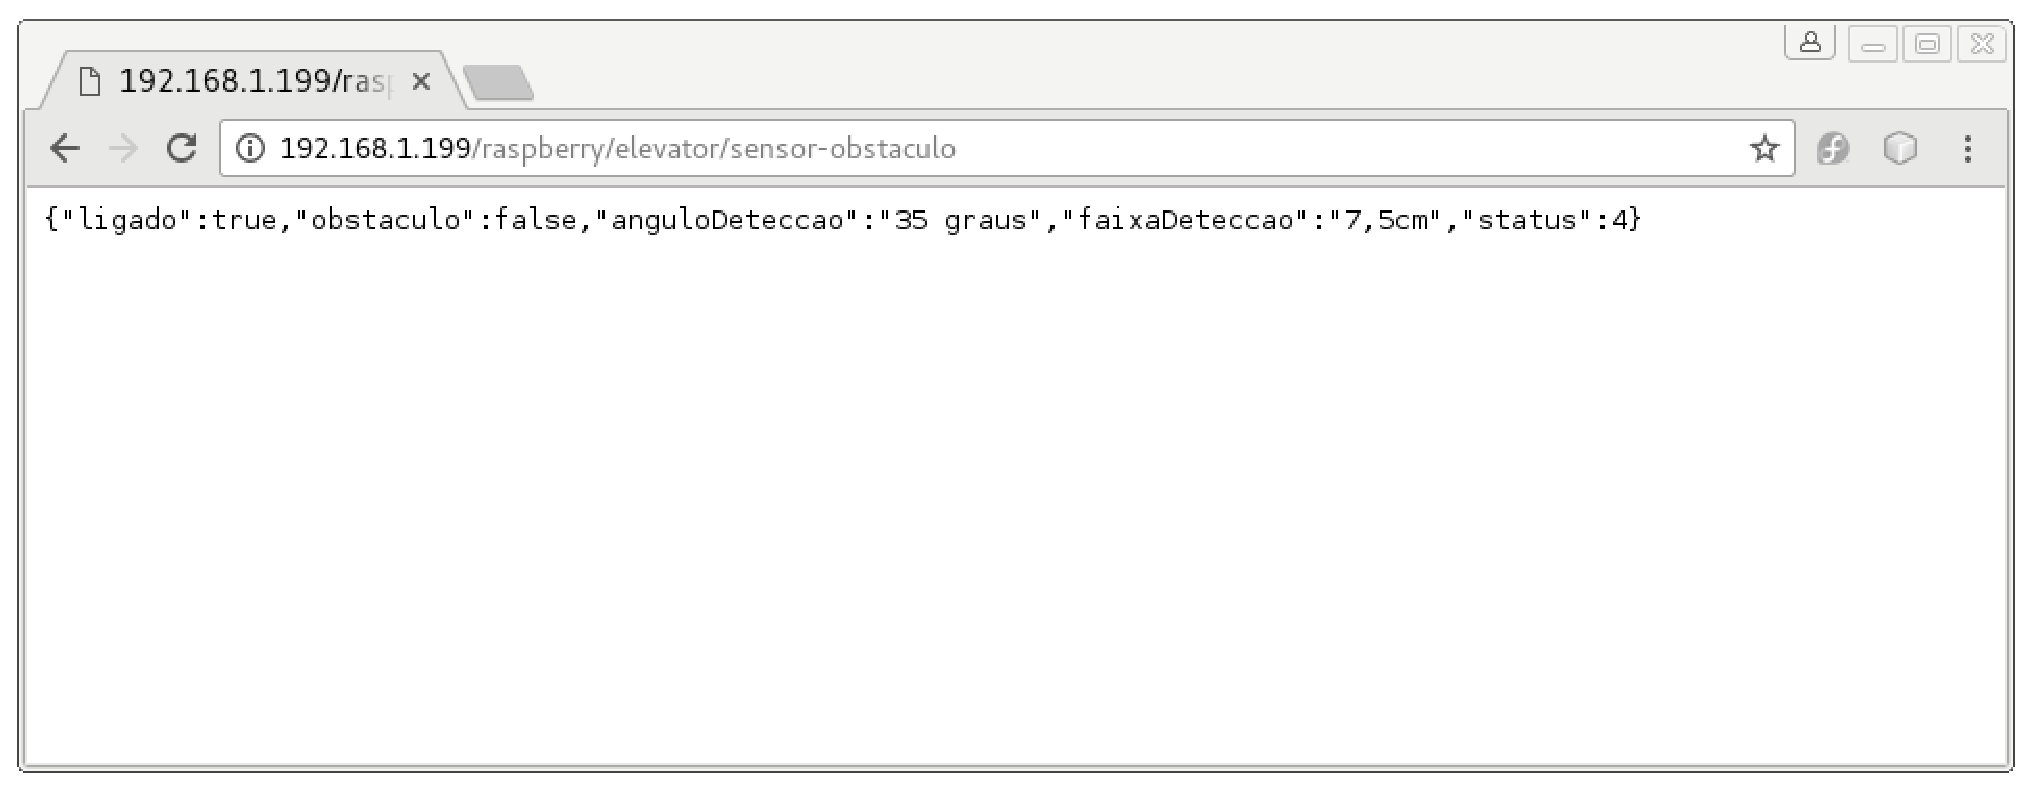
\includegraphics[width=0.8\columnwidth]{fundamentacao/elevator_sensor_example} 
  \caption{Dispositivo sensor de obstaculo do elevador disponibilizado como serviço. Faixa de detecção compatível com a largura do elevador utilizado na maquete do experimento    \ref{ch:experimento}} 
  \label{fig:dispnavegador}
\end{figure}


Nem todos os dispositivos (coisas ou objetos) possuem... TODO RESTxSOAP...

\section{Interação de características}
TODO....origem...causas...etc...
\subsection{Efeitos colaterais desejáveis}
TODO....
\subsection{Efeitos colaterais indesejáveis}
Segundo \cite{Weiss:2007}o problema de efeitos colaterais indesejáveis vem sendo tratado como \textit{the feature interaction problem}.

Em \cite{Weiss}???talvez seja bom mudar esta referencia??? \textit{feature interaction} é definido como a interação entre independentes características***, as quais podem ser intencionais ou não intencionais, podendo levar a efeitos colaterais indesejáveis. Segundo \cite{Weiss:2007 } tais efeitos colaterais indesejáveis podem ser um estado inconsistente do sistema ou inconsistência de dados, tais como, um comportamento não esperado (não desejado), uma quebra de requisito de segurança, dentre outros.

\section{Home network system}
\label{sec:hns}
TODO....

